\documentclass[a4paper, 12pt]{article}
\usepackage{polski}
\usepackage[utf8]{inputenc}
\usepackage{graphicx}
\author{Marcin Fabrykowski}
\title{AIPO\\Laboratorium 03}
\begin{document}
\maketitle
\newpage
\section{Wstęp}
\subsection{Edycja jasności}
Edycja jasności czyli zwiększanie lub zmniejszaie wartości wszystkich pikseli o daną wartość. Minimalna wartość parametru jasności powinna skutkować otrzymaniem obrazu czarnego; maksymalna - obrazu białego.
\subsection{Filtr Sobela}
Filtr Sobela - wykorzystywany przy wykrywaniu krawędzi.
\subsection{Przetwarzany obraz}
Obraz źródłowy znajduje się na rys.~\ref{fig:src}
\begin{figure}[p]

\includegraphics{tux}
\caption{Obraz źródłowy}
\label{fig:src}
\end{figure}
\section{Przetwarzanie obrazu}
\subsection{Zmiana jasności}
Na rys \ref{fig:b-50}, \ref{fig:b-25}, \ref{fig:b25}, \ref{fig:b50}, przedstawiono zmianę jasności obrazu o~odpowienio: -50, -25, 25 oraz 50
\begin{figure}[p]
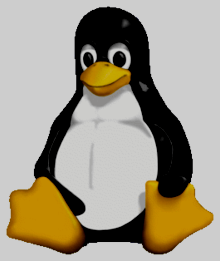
\includegraphics{b-50}
\caption{Zmiana jasności: -50}
\label{fig:b-50}
\end{figure}
\begin{figure}[p]

\includegraphics{b-25}
\caption{Zmiana jasności: -25}
\label{fig:b-25}
\end{figure}
\begin{figure}[p]

\includegraphics{b25}
\caption{Zmiana jasności: 25}
\label{fig:b25}
\end{figure}
\begin{figure}[p]

\includegraphics{b50}
\caption{Zmiana jasności: 50}
\label{fig:b50}
\end{figure}
\subsection{Filtr Robertsa}
Na obrazie \ref{fig:rob} przedstawiony obraz z~nałożonym filtrem Robertsa.
\begin{figure}[p]
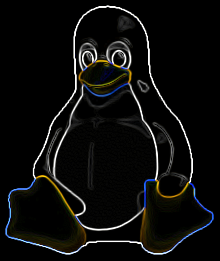
\includegraphics{roberts}
\caption{Filtr Robertsa}
\label{fig:rob}
\end{figure}
\subsection{Filtr Sobela}
Na obrazie \ref{fig:sob} przedstawiony obraz z~nałożonym filtrem Sobela.
\begin{figure}[p]
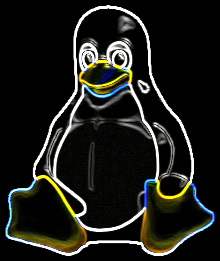
\includegraphics{sobel}
\caption{Filtr Sobela}
\label{fig:sob}
\end{figure}
\subsection{Obrót}
Na obrazie \ref{fig:rot} przedstawiony obraz obrócony o~35 stopni.
\begin{figure}[p]
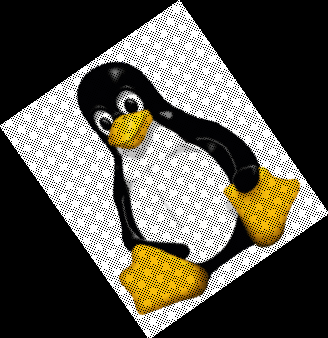
\includegraphics{rot}
\caption{Obrót o~35 stopni}
\label{fig:rot}
\end{figure}
\section{Kod programu}
Z~racji na rozmiar kodu, nie zostanie on wklejony do sprawozdania.\\
Źródła programu zostaną załączone do sprawozdania.
\end{document}
